\documentclass{acmconf}
\usepackage{amssymb}
\usepackage{amsmath}
\usepackage{amstext}
\usepackage{proof}
\usepackage{code}
\usepackage{epsfig}
\usepackage{color}
\usepackage{pstricks,pst-node,pst-tree}

\newcommand{\mygray}{\color{green}}
\newcommand{\mygreen}{\color{green}}

\newcommand{\bangforbindingcolon}{\mathcode`!="003A}
\bangforbindingcolon
\def\sig{\mathsf{sig}}
\def\ctx{\mathsf{ctx}}
\def\kind{\mathsf{kind}}
\def\typeb{\mathsf{type}}
\newcommand{\figfoot}{\vspace{1ex}\hrule}
\newcommand{\fighead}{\hrule\vspace{1.5ex}}

\newcommand{\z}{\mbox{}}

\newcommand{\typeLF}{\textsf{type}}
\newcommand{\propLF}{\textsf{prop}}

\newcommand{\false}{\textsf{false}}
\newcommand{\true}{\textsf{true}}
\newcommand{\andLF}{\; \textsf{and}\;}
\newcommand{\impLF}{\;\textsf{imp}\;}
\newcommand{\forallLF}{\;\textsf{forall}\;}
\newcommand{\existsLF}{\;\textsf{exists}\;}
\newcommand{\eqLF}{\;\textsf{eq}\;}
\newcommand{\eqilLF}{\;\textsf{eqi1}\;}
\newcommand{\eqirLF}{\;\textsf{eqi2}\;}
\newcommand{\eqalLF}{\;\textsf{eqa1}\;}
\newcommand{\eqarLF}{\;\textsf{eqa2}\;}

\newcommand{\andl}{\wedge}
\newcommand{\impl}{\supset}
\newcommand{\ldot}{.\,}
\newcommand{\unif}{\;\doteq\;}

%\newcommand{\andI}{\textsf{andI}}
%\newcommand{\andEL}{\textsf{andE}$_1$}
%\newcommand{\andER}{\textsf{andE}$_2$}
%\newcommand{\impI}{\textsf{impI}}
%\newcommand{\allI}{\textsf{allI}}
%\newcommand{\allE}{\textsf{allE}}
%\newcommand{\orIR}{\textsf{orI}$_1$}
%\newcommand{\orIL}{\textsf{orI}$_2$}
%\newcommand{\orE}{\textsf{orE}}
%\newcommand{\exI}{\textsf{exI}}
%\newcommand{\exE}{\textsf{exE}}
%\newcommand{\impE}{\textsf{impE}}
%\newcommand{\ax}{\textsf{axiom}}
%\newcommand{\trueI}{\textsf{trueI}}
%\newcommand{\falseE}{\textsf{falseE}}

\newcommand{\listd}{\mathsf{list }}
\newcommand{\chars}{\mathsf{char}\;}
\newcommand{\integer}{\mathsf{int}\;}
\newcommand{\nil}{\mathsf{nil}}
\newcommand{\conc}{\;;\;}
\newcommand{\cons}{\mathsf{cons }\;}

\newcommand{\vd}{\vdash}
\newcommand{\vdN}{\Vdash}
\newcommand{\arrow}{\rightarrow}
\newcommand{\hastype}{\mathrel{:}}
\newcommand{\oftp}{\mathord{:}}
\newcommand{\ofvd}{\mathord{::}}
\newcommand{\lam}{\lambda}
\newcommand{\turn}{\mathord{\scriptstyle \vdash}}

\newcommand{\ednote}[1]{\footnote{\it #1}}
\newenvironment{note}{\begin{quote}\message{note!}\it}{\end{quote}}

\newcommand{\lbb}{{[\![}}
\newcommand{\rbb}{{]\!]}}
\newcommand{\Mu}{\lbb M/u\rbb}
\newcommand{\id}{\mathsf{id}}
\newcommand{\msub}[1]{\lbb #1 \rbb}
\newcommand{\inv}[1]{{#1}^{-1}\,}

\newcommand{\type}{\mathsf{type}}
\newcommand{\mctx}{\;\mathsf{mctx}}

\newcommand{\bnfas}{\mathrel{::=}}
\newcommand{\bnfalt}{\mathrel{|}}

\begin{document}
\title{Generating and checking small proof witness for the logical
  framework LF}
\author{Susmit Sarkar and Brigitte Pientka}
\affiliation{}

\maketitle 

\abstract{ Certified code systems demand the production of small-sized
objects which can witness proofs in a machine-verifiable manner. We
present a proof compression and verification engine based on the idea
of giving a proof search procedure hints, which has been called
oracles in the literature~\cite{necula+:oracles}.  The new features in
our system are that ours is a general purpose utility, not specialised
to any particular logic. Further, we integrate our tool with the Twelf
system, which has been widely used for certified code systems. We use
techniques from tabled logic programming to further reduce the size of
our proof witnesses. }

\section{Introduction}
Proof-carrying code applications establish trust by verifying
compliance of the code with safety and security policies.
A code producer verifies that the program is safe to
run according to some predetermined safety policy, and supplies a
binary executable together with its safety proof. Before
executing the program, the code consumer then quickly checks the code's
safety proof against the binary. 

Many proof-carrying code projects, in particular in foundational PCC,
have employed the logical framework LF as a general safety
infrastructure for encoding safety polcies and representing safety
proofs\cite{AppelFelty00,Crary:POPL03,AppelFelten99,Crary:CADE03}.
The main advantage of using a logical framework is its flexibility
and its smal trusted computing base. Hence, it reduces the effort
required for each particular safety policy. However, proofs within the
logical framework may be large in size 
% several mega-bytes - with LFi few tens of kilobytes (=two orders of
% magnitude) 
, e.g. 4-times as big as the
actual machine code. This has spawned a number of research
contributions to reduce proof size and proof checking time for
proof-carrying code applications. However, all these contributions
trade the expressive power and complexitity of LF against
simplicitiy. In a first step, Necula and Lee's \cite{Necula98lics} developed a
proof representation for LF$_i$, essentially a restriction to 2-level
logical framework, which eliminated many implicit type information in
the representation of proofs. However, proofs in LF$_i$ are still
4-times as big as the program they are certifying.
To obtain even smaller proofs (1/8th the size of the machine code),
Necula proposed in \cite{Necula+01:oracle} to only record the
non-deterministic choices which were made when constructing the proof,
and then use a guided prover to reconstruct the proof on the consumer
side. This simple idea has been proven to be effective in many
practical examples, and most recently has been proposed within the
Open Verifier Framework \cite{Necula}. Appel et al. use a similar idea
for creating a foundational proof checker with small
witnesses. However, all these approaches are restricted to simply 
typed Prolog-like engines. The beauty and power of logical frameworks
is traded for simplicity. This is unfortunate since higher-order
features, which are often used when encoding safety logics and type systems,
need to be encoded or circumvented using tricks or are simply
disallowed. As we move beyond proving memory safety, we predict that
richer safety logics and type systems which benefit from the full
power provided by LF will play a more important role in proof-carrying
code applications. Hence the need for general purpose proof-checkers
for full LF will grow.

In this paper, we describe the design of a oracle-based proof checker for
full LF. This demonstrates that many of the existing restrictions
which are placed on oracle-based proof checkers are unnecessary. The
main obstacle in building a oracle-based proof checker for full LF
is due to higher-order terms (e.g. terms my contain
$\lambda$-abstraction). As a consequence, known oracle-based proof checking
systems entirely avoid this problem and concentrate on the first-order
fragment, where for example unification is decidable and easily
implemented and efficient term indexing operations are known to make
it practical. In this paper, we show that this restriction to
first-order terms is unnecessary. Moreover we demonstrate it is
possible to extend Twelf with making it unnecessary to build seperate
proof checking engines.
We propose the use of higher-order substitution tree indexing together
with linear higher-order pattern unification to extend oracle-based
proof checking to the higher-order setting. Furthermore, we improve on
the size of oracle-proofs by factoring out common
sub-proofs\footnote{Eliminating common sub-proofs   is an orthogonal
  problem to eliminating redundant implicit type 
  information, as is   proposed in \cite{Necula98lics}.} by
incorporating memoization techniques. Identifying and factoring out
common sub-proofs leads to more compact oracles and can potentially
decrease proof-checking time since common sub-proofs are only checked once. 

We hope this will provide a comprehensive guide for future
implementations of proof checkers which need not be restricted to
first-order prolog-like systems. In particular, various
certified code systems can exploit this idea. However, small proof
witnesses not only play a role in certifiyng code, but are useful and
sometimes necessary in building in certifying theorem proving and
logic programming engines. First, constructing and possibly storing
full proof terms may be expensive, hence witnesses provide a cheap
simple alternative. As an example consider tabled higher-order logic
programming, where we memoize subgoals together with their answers and
proofs to re-use the results later. Constructing and storing the full
proof term however would impose a substantial performance
penalty. Hence, small witnesses in forms of oracles  provide a cheap
simple alternative and are in fact crucial to obtain a practical
tabled logic programming interpreter. Second, there has been interest
in producing proof justifiers in the logic programming community to
ease debugging. Small proof witnesses can be viewed as proof
justifiers and may be used to re-trace the proof. We have implemented
a oracle-based proof generator and checker as part of the logical
framework {\em Twelf}.  

The paper is structured as follows. We give background on
higher-order logic programming in Twelf in Section~\ref{sec:twelf}. In
Section~\ref{sec:oracles}, we present our approach to oracle-based
proof generation and proof checking. In particular, we explain
higher-order term indexing to index higher-order logic programming
clauses. In Section~\ref{sec:tabling}, we discuss memoization techniques for
factoring out common subproofs. We conclude with a discussion of some
experimental results within Twelf and discussion of related work.

\section{Higher-order logic programming}\label{sec:twelf}

Higher-order logic programming extends first-order logic programming
in three main ways: First, first-order terms are replaced with
(dependently) typed $\lambda$-terms. Second, the body of clauses may
contain implications and universal quantification, thereby generating
dynamic assumptions which may be used during proof search. Thirdly,
execution of a query will not only produce a yes or no answer, but
generate a proof term as a certificate which can be checked
independently. These features make higher-order logic programming an
ideal generic framework for implementing formal safety policies given via
axioms and inference rules and executing them.

The theoretical foundation underlying higher-order logic programming
within Twelf is the LF type theory, a dependently typed lambda
calculus. We will first give an example of encoding the natural
deduction calculus in the logical framework LF using higher-order
logic programming following the methodology in  \cite{harper+:lf}. For
more information on how to encode formal systems in LF see
\cite{Pfenning97}. 

Using this example, we will explain oracle-based proof generation and
proof-checking. 

\subsection{Representing Logics}
As a running example, we will consider intuitionistic propositional
logic formulated in the natural deduction style. We assume two atomic
propositions, truth and falsehood, and we will allow conjuction,
disjunction, and implication as connectives. First-order ogic can be
characterized as follows: 
\[
\begin{array}{llll}
\mbox{Propositions} & A,B, C & := & \true \mid \false \mid A \andl B
\mid A \impl B \\
& & & \mid \forall x.A \mid \exists x.A\\
\mbox{Context} & \Gamma & := & \ldot \mid \Gamma,  A
\end{array}
\]

Inference rules describing natural deduction are presented in Table~\ref{natded}.

\begin{table}[h]
\fighead
\[
\infer{\Gamma\vdash \forall x. A}
{\Gamma\vdash [a/x]A & a \mbox{ is new}}
\qquad
\infer{\Gamma\vdash [T/x]A}
{\Gamma\vdash \forall x.A}
\]
\[
\infer{\Gamma\vdash A\supset B}
{\Gamma,A\vdash B}
\qquad
\infer{\Gamma\vdash B}
{\Gamma\vdash A\supset B
\quad
\Gamma\vdash A}
\]
\[
\infer{\Gamma\vdash A\wedge B}
{\Gamma\vdash A\quad \Gamma\vdash B}
\qquad
\infer{\Gamma\vdash A}
{\Gamma\vdash A\wedge B}
\qquad
\infer{\Gamma\vdash B}
{\Gamma\vdash A\wedge B}
\]
\[
\infer{\Gamma\vdash A\vee B}
{\Gamma\vdash A}
\qquad
\infer{\Gamma\vdash A\vee B}
{\Gamma\vdash B}
\]
\[
\infer{\Gamma\vdash C}
{\Gamma\vdash A\vee B
\quad
\Gamma,A\vdash C
\quad
\Gamma,B\vdash C
}
\]
\[
\infer{\Gamma\vdash\top}
{}
\qquad
\infer{\Gamma\vdash C}
{\Gamma\vdash\perp}
\qquad
\infer{\Gamma, A \vdash A}
{}
\]
\caption{\label{natded}A natural deduction system}
\figfoot
\end{table}

To represent this system in LF, we first need formation rules to
construct terms for the objects we are talking about, in this case,
propositions. We declare a new type {\tt prop} for propositions and a
type {\tt i} for individuals. We intend that terms belonging to {\tt
  prop} represent well-formed propositions. The rules are given below,
in concrete Twelf syntax. 

\begin{code}
prop : type.
i    : type.
\vspace{0.1in}
true   : prop.
false  : prop.
and    : prop -> prop -> prop.
or     : prop -> prop -> prop.
imp    : prop -> prop -> prop.
forall : (i -> prop) -> prop.
exists : (i -> prop) -> prop.
\end{code}

The connectives for conjunction, disjunction and implication are
mapped to constructors taking two propositions and returning a
proposition. To represent bound variables in the forall- and
exists-quantifier, we use higher-order abstract syntax. The crucial
idea is to represent bound variables in the object language (logic)
with bound variables in the meta-language (higher-order logic
programming). 

Next we turn our attention to the proofs in our system. We have a
judgment for provability within this logic. We map this judgment to
a type family {\tt prov}, which has a (dependent) kind.

\begin{code}
prov : prop -> type.
\end{code}

Each clause will correspond to an inference rule in the object
logic. For convenience, we give the constructors 
descriptive names, and follow the order of the rules in
Table~\ref{natded}. 

\begin{code}
foralli   : prov (forall $\lambda$x. A)
            <- $\Pi$x. prov (A x)
foralle   : prov (A T)
            <- prov (forall $\lambda$x. A).
\z
impi     : prov (imp A B)
            <- (prov A -> prov B).
impe     : prov B
            <- prov (imp A B)
            <- prov A.
\z
andi     : prov (and A B)
            <- prov A
            <- prov B.
ande1    : prov A
            <- prov (and A B).
ande2    : prov B
            <- prov (and A B).
\z
ori1     : prov (or A B)
            <- prov A.
ori2     : prov (or A B)
            <- prov B.
ore      : prov C
            <- prov (or A B)
            <- (prov A -> prov C)
            <- (prov B -> prov C).
\z
truei    : prov true.
\z
falsee   : prov C
            <- prov false.
\end{code}

These rules are given as a Twelf signature. $A$, $B$, $C$ denote logic
variables which are instantiated during proof search. 
There are two key ideas which make the encoding of the sequent
calculus elegant and direct. First, we use higher-order abstract
syntax to encode the bound variables in the universal and existential
quantifier. Second, we use the power of dynamic assumptions which
higher-order logic programming provides, to eliminate the need to
manage assumptions in a list explicitely. To illustrate, we consider the
clause {\tt impI}. To  prove {\tt prov (A => B)}, we prove {\tt prov B}
assuming {\tt prov A} In other words, the proof for $prov B$ may use
the dynamic assumption $prov A$. 

\subsection{Higher-order logic programming}

Higher-order logic programming is similar to a Prolog interpreter
since it performs essentially a depth-first search over all the
program clauses. However, in the higher-order setting we may have
dynamic assumptions which may be used within a certain
scope. Moreover, since Twelf allows higher-order terms (i.e. terms may
contain $\lambda$-abstraction), higher-order unification is used to
unify clause heads with current goal. Finally, proof terms are
generated.

We will illustrate the process by showing proof search for the
proposition {\tt prov (imp true (imp (imp true false) false))}
(corresponding to $(\top \supset ((\top \supset \perp) \supset
\perp))$) works.  The proof tree for this is shown in
Figure~\ref{prooftree1}.

\begin{figure}
\fighead
\epsfig{file=prooftree1.ps,width=2.7in}
\caption{\label{prooftree1} Proof Tree for 
$\top\supset((\top\supset\perp)\supset\perp)$}
\figfoot
\end{figure}
      
We notice that it is of the form {\tt prov (imp A B)}, so various clauses
apply. We pick the first of these applicable clauses ({\tt
impi}). This instantiates {\tt A} to {\tt true}, and {\tt B} to {\tt
(imp (imp true false))}.  If this clause succeds producing the proof
$P$, we want to emit the proof {\tt impi (true) (imp (imp true false))
$P$}.  There is only one subgoal, which involves making the dynamic
assumption {\tt prov true}, and then trying to solve {\tt prov (imp
(imp true false) false)}. This means that we want to come up with a
proof term for {\tt prov~(imp~(imp~true~false)~false)} with {\tt
x$!$prov true} in the context, where $x$ is a new variable. From an
operational view point, the search can be described as follows:

\fighead
\begin{small}
Solve Goal $\Gamma \vd G$:
\begin{enumerate}
\item \mbox{Given an atomic goal $P$ in dynamic context $\Gamma$:}\hfill\\
     look through the program $\Gamma$ to establish a proof for $P$.

\item Given goal $A_1 \arrow A_2$, add the dynamic assumption $A_1$ to the
  programs in $\Gamma$ and attempt to solve the goal $A_2$ from the extended
  program $\Gamma, c\oftp A_1$.
\item Given a universally quantified goal $\Pi x\oftp A_1. A_2$, we
     generate a new parameter $c$, and attempt to solve $[c/x]A_2$ in the
    extended program context $\Gamma, c\oftp A_1$.
\end{enumerate}
\end{small}
\figfoot 

Once the goal is atomic, we need to select a clause from the
program context $\Gamma$ to establish a proof for $P$. In a logic
program interpreter, we consider all the clauses in $\Gamma$ in order. 
First, we will consider the dynamic assumptions, and then we will try
the static program clauses one after the other. 
Let us assume, we picked a clause $A$ from the program context
$\Gamma$ and we now need to establish a proof for $P$.

\fighead
\begin{small}
Focus on clause $A$ to solve atomic goal $P$.
\begin{enumerate}
\item Given the atomic clause $P'$ with name $n$, we establish a proof for the
  atomic goal $P$ by checking if $P'$ unifies with $P$. If yes then
  succeed. Otherwise fail and backtrack. 
\item Given the clause $A_2 \arrow A_1$ with name $n$, we attempt to establish a
  proof of the atomic goal $P$, by trying to use the clause $A_1$ to
  establish a proof for $P$. If it succeeds attempt to solve the goal
  $A_2$. If it fails,  backtrack. 
\item Given the clause $\Pi x\oftp A_1. A_2$ with name $n$, we
  establish a proof for the atomic goal $P$ by generating a new logic
  (existential) variable $u$, and use the clause $\msub{u[\id]/x}A_2$
  to establish a proof for the atomic goal $P$. 
\end{enumerate}
\end{small}
\figfoot

The proof search continues searching the tree in the figure, eventually 
succeeding. The corresponding answer term (in implicit form) is 
\begin{code}
(impi ([x:prov true] impi 
       ([y:prov (imp true false)] impe x y))).
\end{code}

For illustration, the explicit answer term, which does not require type
reconstruction to instantiate implicit parameters, is 
\begin{code}
impi true (imp (imp true false) false)
    ([x:prov true]
        impi (imp true false) false
            ([y:prov (imp true false)] 
                impe true false x y)).
\end{code}

We see that assuming we have type reconstruction at the verifier has
led to proof terms which are smaller, but still quite big.

Our goal is to reduce the proof evidence to the non-deterministic
choices we have made during the proof to produce small proof witnesses. 
      
\section{Oracle-based proof search}
\label{sec:oracles}

In this section, we describe the oracle-based proof generation and
checking. To generate oracles we can follow two ways. First, we may
use any logic-programming proof search procedure available to generate
a bit-string during proof search. This may in general not be feasible,
although it can be often done with more sophisticated theorem proving
technology. In certifying code systems however the safety proof is
usually generated by a certifying compiler, and we merely aim at
compressing the safety proof into a bit-string.

\subsection{Generating small proof witnesses}

We will modify the verifier's proof search procedure to execute as in
the previous section, with the addition that whenever it faces a
non-deterministic choice, it will generate a bit-string which
corresponds to its successful choice. 

\fighead
\begin{small}
Solve Goal $\Gamma \vd G$:
\begin{enumerate}
\item \mbox{Given an atomic goal $P$ in dynamic context
    $\Gamma$:}\hfill\\
  \begin{enumerate}
  \item look through the dynamic assumptions $\Gamma$ to establish a proof for $P$ 
  \item Extracting all clauses $\Pi x_1\oftp B_1\ldots.Pi x_k\oftp
    B_k. A_n \rightarrow \ldot A_1 \rightarrow P'$ with name $n$,
    whose head $\msub{u_1[\id]/x_1, \ldots u_k[\id]/x_k}P'$ unifies
    with $P$ under $\theta$. Try all these applicable clauses in
    order and establish proofs for all the subgoals
    $\msub{\theta}A_1, \ldots, \msub{\theta}A_n$ of applicable clause
    $n$. If the $i$-th clause succeeds from $n$ applicable clauses and
    returns witness $w$, then return the new witness $i . w$.
  \end{enumerate}

\item Given goal $A_1 \arrow A_2$, add the dynamic assumption $A_1$ to the
  programs in $\Gamma$ and attempt to solve the goal $A_2$ from the extended
  program $\Gamma, c\oftp A_1$.
\item Given a universally quantified goal $\Pi x\oftp A_1. A_2$, we
     generate a new parameter $c$, and attempt to solve $[c/x]A_2$ in the
    extended program context $\Gamma, c\oftp A_1$.
\end{enumerate}
\end{small}
\figfoot 

Once the goal is atomic, we need to select a clause from the
program context $\Gamma$ to establish a proof for $P$. In a logic
program interpreter, we consider all the clauses in $\Gamma$ in order. 
First, we will consider the dynamic assumptions, and then we will try
the static program clauses one after the other. For proof generation,
we need to be able to pre-select all clauses whose head unifies with
the current goal.

The key insight is that proof search is deterministic, if we know what
program clause or dynamic clause to pick for each subgoal (see the
procedure for solving goal $A$ from clauses in $\Gamma$, step 1). Let
us briefly consider an example to illustrate. To prove

\[
(\top\!\supset\!((\perp\!\wedge\!\perp)\!\supset\!%
((\perp\!\wedge\!\top)\!\supset\!\perp)\!\supset\!\perp))
\]

A prover must consider the following choices.
At the top level, we have to prove an implication. 5 choices apply
(implication introduction and all four eliminations), and we should
take the first one. In general, a theorem prover which is searching for a
proof may explore several non-successful branches, until finding the
right choice. Now we have to prove
$((\perp\wedge\perp)\supset(((\perp\wedge\top)\supset\perp)\supset\perp))$,
and we add $\top$ to our dynamic list of assumptions.

At the next stage, 6 choices apply (all the previous ones, and also a
dynamic assumption). The first choice would have
been the dynamic assumption, which should eventually fail.
The second one (implication introduction) proves to be successful. Now we
have to prove $((\perp\wedge\top)\supset\perp)\supset\perp)$ and we add
$(\perp\wedge\perp)$ to our dynamic list of assumptions.

This process continues to eventually find the proof. The list of
choices made in this proof search procedure is $1/5$, $2/6$, $3/7$,
$4/7$, $1/8$, $5/8$, $5/7$, $2/7$, and $3/7$, keeping in mind that
dynamic assumptions are tried first by proof search procedures.      
This sequence is all that needs to be generated and sent to the
verifier. 
      
This sequence is all that needs to be sent to the verifier. The
verifier has to perform the proof search procedure as outlined
above. Whenever there is a choice to be made, she looks at the next
advice and takes the appropriate branch.

This leads to an efficient encoding of the choices. If we have $k$
choices, we need $\lceil\log_2 k\rceil$ bits. Since we know that the
path through the proof tree always has to lead to a proof, if there is
only one choice applying, this formula correctly says that we do not
need to emit an advice.  The verifier knows how many choices apply, so
she can calculate the number of bits to pick off the oracle. This
means that we do not need an explicit separator between the choices.

As we mentioned previously, sometimes finding a proof automatically
may be hard and infeasible. Moreover, in certifying code we in fact
have a safety proof generated by the compiler and we can compress the
proof term into an oracle by guiding the prover with the proof term.

\begin{note}
  Does a certifying compiler really output LF proof terms??? -- Why
  doesn't it output oracles directly?
\end{note}

The explicit proof term for the previous statement is as follows:
 
\begin{code}
impi ([x1:prov true] 
    impi ([x2:prov (and false false)]
           impi 
               ([x3:prov (imp (and false true) 
                    false)]
               (impe (andi x1 (ande1 x2)) 
                    x3))))
\end{code}

For the idea to work, proof witness generation and witness checking
have to perform essentially the same overall proof search. Moreover,
the order in which different choices are considered must be the same.
The only difference is that during witness generation we would explore
possible multiple fruitless paths until settling on the right one,
while in witness checking we know by inspecting the advice encoded in
the bit-string which choice to consider.

\subsection{Checking small proof witnesses}
In this section, we modify the previous search procedure, in such a
way that it does not search for the correct choice, but takes into
account the advice from the bit-string on how to proceed. 

To check that proof witnesses in fact constitute a valid proof for a
given proposition, we re-run the prover guided with the advice encoded
in the bit-string. The witness checker is then in fact a deterministic
search procedure. No backtracking is necessary, since all the
non-deterministic choices are resolved.  By taking the appropriate
branches (and performing the needed substitutions of universal
variables by unification), the user can be convinced that such a
proof exists. This can lead to savings of time and memory.
This however requires the code consumer to trust the witness
checker. For a paranoid consumer this may be unacceptable since the witness
checker may use optimizations such as caching subproofs and indexing,
which can be quite complicated. In this case, it is possible to also
decompress the proof witness to an explicit proof term and use a different
trusted type-checker to verify the expanded proof witness.

\section{Optimizations: Higher-order Term Indexing}

A proof search procedure must have a way of retrieving all clauses of
the logic program which may satisfy the current goal, since such a
method will dictate how many choices we are returned at any step, and
hence is critical in understanding the oracle. Most first-order logic
programming interpreter use term indexing strategies to efficiently
retrieve all clauses whose head unifies with the current goal.

In the higher-order setting, much fewer indexing strategies exist for
higher-order terms and are not generally known. For the purpose of
this paper, we will adopt higher-order substitution trees as described
in \cite{Pientka:ICLP03}.Substitution tree indexing has been
successfully used in a first-order setting \cite{graf:substtrees} and
allows the sharing of common sub-expressions via substitutions. This
is unlike other non-adaptive term indexing, which only allow sharing
of common term prefixes. 

To appreciate the difficulties in higher-order term indexing and
understand why all existing witness generation and checking procedures
avoid it, we briefly summarieze the main challenges:
 First of all, building a substitution tree relies on computing the
 most specific generalization of two terms. However in the
 higher-order setting, the most specific generalization of two terms (heads)
 does not exist in general. Second, retrieving all heads, which unify
 with the current goal, needs to be efficient --
but higher-order unification is undecidable in general.  As discovered
by Miller \cite{Miller91iclp}, there exists a decidable fragment,
called higher-order patterns. For this fragment, unification and
computing the most specific generalization is decidable even in 
rich type theories with dependent types and polymorphism as shown by
Pfenning \cite{Pfenning91lics}.  However, these algorithms may not be
efficient in practice  \cite{PientkaPfenning:CADE03} and hence it is
not obvious that they are suitable for higher-order term
indexing techniques. 

In \cite{Pientka:ICLP02}, we propose substitution tree indexing for
higher-order terms based on linear higher-order patterns. Linear
higher-order patterns refine the notion of higher-order patterns
further and factor out any computationally expensive parts. As shown
in \cite{PientkaPfenning:CADE03}, many terms encountered fall into
this fragment and linear higher-order pattern unification performs well in
practice. In \cite{Pientka:ICLP02,Pientka:Phd}, we give a formal
description for computing the most specific generalization of two
linear higher-order patterns, for inserting terms in the index and for
retrieving a set of terms from the index s.t. the query is an instance
of the term in the index, and show correctness. This can be extended
to unifiability. For this setup to work cleanly in the higher-order
setting, it is crucial that we distinguish between existential
variables in $\Delta$ and bound variables and assumptions in
$\Gamma$. Moreover, it is essential that existential variables allow
in place up-date. In particular, we will rely on the notion of
existential variables which are ``fully applied'', i.e. they may
depend on all the bound variables they occur in.

 In the following, we will describe requirements and
challenges we face of memoizing sub-goals in the higher-order setting. 


\[
\begin{array}{ll}
\eqLF: & \propLF \rightarrow \propLF \rightarrow \typeLF.\\[1em]
%
\eqilLF: & \eqLF (\forallLF \lambda x. \impLF (A\; x)\; B)\quad (\impLF (\existsLF \lambda x. A\; x)\; B).\\
\eqirLF: & \eqLF (\forallLF \lambda x. \impLF A \; (B\; x)) \quad (\impLF A\; (\forallLF \lambda x. B\;x)).\\
\eqalLF: & \eqLF (\forallLF \lambda x. \andLF (A\; x)\; B) \quad (\andLF (\forallLF \lambda x. A \;x) \; B).\\
\eqarLF: & \eqLF (\forallLF \lambda x. \andLF A \; (B\;x)) \quad (\andLF A \; (\forallLF \lambda x. B\; x)).\\
\end{array}
\]

After linearization:
\[
\begin{array}{ll}
\eqLF: & \propLF \rightarrow \propLF \rightarrow \typeLF.\\[1em]
%
\eqilLF: & \eqLF (\forallLF \lambda x. \impLF (A'\; x)\; (B'\;x)\quad (\impLF (\existsLF \lambda x. A\; x)\; B). \\
         & \forall x. (A'\; x) \unif (A \; x) {\textsf{ and } } B'\;x   \unif B\\[0.5em]
\eqirLF: & \eqLF (\forallLF \lambda x. \impLF (A'\;x) \; (B'\; x)) \quad (\impLF A\; (\forallLF \lambda x. B\;x)).\\
         & \forall x. (A'\; x) \unif A  {\textsf{ and }} B'\;x   \unif (B\;x)\\[0.5em]
\eqalLF: & \eqLF (\forallLF \lambda x. \andLF (A'\; x) \; (B'\;x)) \quad (\andLF (\forallLF \lambda x. A \;x) \; B).\\
         & \forall x. (A'\; x) \unif (A \; x) {\textsf{ and }} B'\;x   \unif B\\[0.5em]
\eqarLF: & \eqLF (\forallLF \lambda x. \andLF (A'\;x) \; (B' x)) \quad (\andLF A \; (\forallLF \lambda x. B\; x)).\\
         & \forall x. (A'\; x) \unif A  {\textsf{ and }} B'\;x   \unif (B\;x)\\[0.5em]
\end{array}
\]


%
% eqi1: eq (forall $\lambda$ x. imp (A' x) (B' x)) (imp (exists $\lambda$ x. A x) B).
% residual equations: B' x = B    A' x = A x

% eqi2: eq (forall $\lambda$ x. imp (A' x)  (B' x)) (imp A (forall $\lambda$ x. B x)).
% residual equations: B' x = B x    A' x = A

% eqa1: eq (forall $\lambda$ x. and (A' x)  (B' x)) (and (forall $\lambda$ x. A x) B).
% residual equations : A' x = A x   B' x = B

% eqa1: eq (forall $\lambda$ x. and (A' x)  (B' x)) (and A (forall $\lambda$ x. B x)).
% residual equations: B' x = B x    A' x = A
%
%
%
%
% \begin{small}
\begin{figure*}[htbp]
  \begin{center}
    \begin{small}
\pstree[nodesep=1pt,levelsep=9ex]{%
\TR{$\eqLF (\forallLF \lambda x. i_1[\id]) \quad i_2[\id]$} }{%
  \pstree{\TR{\begin{tabular}{r}
              $(\andLF A'[\id]\; B'[\id])/i_1$\\
              $(\andLF i_3[\id]\; i_4[\id])/i_1$\\
            \end{tabular}
          }
        }{%
          \pstree{\TR{\begin{tabular}{r}
                $\forallLF \lambda x. A[\id]/i_3$,\\
                $B/i_4$
              \end{tabular}
            }}{%
            \pstree{\TR{\begin{tabular}{l}
                  $A'[\id]\unif A[x/x]$\\
                  $B'[\id]\unif B$
                \end{tabular}
              }}{ $\eqarLF$}
          }
%
          \pstree{\TR{\begin{tabular}{r}
                $A/i_3,$\\
                $\forallLF \lambda x.B[\id]/i_4$
              \end{tabular}
            }
          }{%
            \pstree{\TR{\begin{tabular}{l}
                $A'[\id]\unif A$\\
                $B'[\id] \unif B[\id]$
              \end{tabular}
            }
            }{ $\eqalLF$}
          }
        }
%%%%% second child
          \pstree{\TR{\begin{tabular}{r}
                     $(\impLF A'[\id]\; B'[\id])/i_1$\\
                     $(\impLF i_3[\id]\; i_4[\id])/i_2$\\
                   \end{tabular}
                 }}{
                 \pstree{\TR{\begin{tabular}{r}
                       $\forallLF \lambda x. A[\id]/i_3$,\\
                       $B/i_4$
                       \end{tabular}
                     } }{%
                     \pstree{\TR{\begin{tabular}{l}
                           $A'[\id]\unif A[x/x]$\\
                           $B'[\id]\unif B$
                         \end{tabular}}
                     }{$\eqirLF$}
                   }
                  \pstree{\TR{\begin{tabular}{r}
                        $A/i_3,$\\
                        $\forallLF \lambda x.B[\id]/i_4$
                      \end{tabular}}}{
                    \pstree{\TR{\begin{tabular}{l}
                          $A'[\id]\unif A$\\
                          $B'[\id] \unif B[\id]$
                        \end{tabular}}
                    }{$\eqilLF$}
                  }
                }
              }
        
    \end{small}
  \end{center}
  \caption{Substitution tree}
  \label{fig:substree}
\end{figure*}

% \end{small}

In contrast to other indexing techniques such as discrimination tries,
substitution trees  allows the sharing of common sub-expressions
instead of common term prefixes.

This is especially important for indexing dependently typed terms. 

\begin{note}
  Give an example? -- for example, annotate every formula with its size?
\end{note}

We have chosen to index only the static set of program clauses. In
theory, it is possible to use substitution tree indexing for dynamic
clauses generated during proof search.  However, it is not clear how
useful this will be, since the process of creating the tree itself is
time-consuming. It is also noted by Necula and Rahul \cite{} that
indexing dynamic assumptions imposes a performance penally. It is
useful to pre-process the program, but the payoff with dynamic clauses
is unclear. For dynamic clauses, we use only simple head term matching.


\section{Caching results}
\label{sec:tabling}
Since large proofs often have identical subproofs,  there is a
lot of opportunity for sharing subproofs. The problem is particularly
acute in machine-generated proofs for certifying machine-code which
tend to have repeated proofs of simple facts. This problem has been
already pointed out by Necula and Lee in \cite{NeculaLee+97:resource}

 \begin{tabular}[h]{l}
``...it is very common for the proofs to have  \\
repeated sub-proofs that should be hoisted out and \\
proved only once ...'' \cite{NeculaLee+97:resource}\\ $\;$
 \end{tabular}


In the context of oracle-based proof checking, this leads to two
problems.  First, the oracles become larger in size than
necessary. This means that what has to be transmitted to the verifier
is large in size. Secondly, the performance of witness checker may
degrade, since it spends its time uselessly proving the same fact over
and over again. 

Ideally we would like to cache intermediate results and re-use them
later. Up to now, this has been difficult since we need to efficiently
store and retrieve intermediate goals. We re-use and build upon recent
work \cite{pientka:tabled} on memoizing intermediate goals during
execution as part of the tabled higher-order logic programming and
adapt it for witness generation and witness checking. 

When we generate compressed witnesses from explicit proof terms or
when we check compressed witnesses, we have the advantage that we know
a proof exists. This is simplifies memoization substantially, since we
can add the goal together with its answer substitution and proof
witness into a memo-table once we have finished proving it. We modify
again the first step of the proof. First, we will check if there
exists already an answer toghether with a proof witness in the memo-table for
the current goal $\Gamma \vd G$. If there exists such an answer we
will re-use it and return the proof witness. 
Second, we will destructively update the memo-table when we have
proven a goal. In addition to returning the proof witness $i . w$, we
destructively update the memo-table, by adding the current goal
$\Gamma \vd G$ together with its answer substitution and proof witness
$i . w$.  

\fighead
\begin{small}
Solve Goal $\Gamma \vd G$:
\begin{enumerate}
\item \mbox{Given an atomic goal $P$ in dynamic context
    $\Gamma$:}\hfill\\
  \begin{enumerate}
  \item look through the dynamic assumptions $\Gamma$ to establish a proof for $P$ 
  \item Extracting all clauses $\Pi x_1\oftp B_1\ldots.Pi x_k\oftp
    B_k. A_n \rightarrow \ldot A_1 \rightarrow P'$ with name $n$,
    whose head $\msub{u_1[\id]/x_1, \ldots u_k[\id]/x_k}P'$ unifies
    with $P$ under $\theta$. Try all these applicable clauses in
    order and establish proofs for all the subgoals
    $\msub{\theta}A_1, \ldots, \msub{\theta}A_n$ of applicable clause
    $n$. If the $i$-th clause succeeds from $n$ applicable clauses and
    returns witness $w$, then return the new witness $i . w$.
  \end{enumerate}
\end{enumerate}
\end{small}
\figfoot

\begin{note}
  Say how to store elements in a table.
The table setup is as follows:
\[
\begin{array}{ll}
\mbox{Table entry} & \Delta ; \Gamma \vd G\\
\mbox{Residual Equ.} & \Delta ; \Gamma \vd R \\
\mbox{Answer substitution} & \Delta' \vd \theta : \Delta
\end{array}
\]

Apply strengthening to detect more identical subproofs (strengthening
based on subordination and on not adding dynamic assump twice)
The design supports naturally substitution factoring based on explicit
substitutions\cite{RamakrishnanJLP99}. With substitution factoring the
access cost is proportional to the size of the answer substitution
rather than the size of the answer itself\footnote{may not be necessary in
this setting -bp?}
\end{note}

The stored solution to a tabled goal is not always the solution we
want to use.  This is because using a particular answer will constrain
the free variables, possibly in ways not helpful to the proof. 

We add the choices from the table to the menu of choices available at
every choice point. Again, both the prover and verifier are following
similar algorithms, so both have identical caches. The number of
choices is also the same in both the prover and verifier. We just need
a convention on how to specify a tabled answer, and we choose the
choices appearing in the table to precede the other choices.

\begin{figure}
\fighead
\hspace{-0.5in}
\psfig{file=prooftree3.ps,width=2.7in,height=2.5in}
\vspace{1.5in}
\caption{\label{prooftree3}
$(\top\supset((\top\supset\perp)\supset\perp) \wedge
(\top\supset((\top\supset\perp)\supset\perp)$}
\figfoot
\end{figure}

To take an example, look at the proposition
$(\top\supset((\top\supset\perp)\supset\perp) \wedge
(\top\supset((\top\supset\perp)\supset\perp)$, whose proof tree is
given in Figure~\ref{prooftree3}. Notice the common subtrees marked
with dotted lines.  In the absence of caching results, the sequence of
choices would be 3/5, 1/5, 2/6, 3/6, 1/7, 2/6, 1/5, 2/6, 3/6, 1/7, and
2/6. With caching of results, we get the substantially shorter oracle
3/5, 1/5, 2/6, 3/6, 1/7, 2/6, and 1/6.

\section{Related Work}
The idea of using oracles in proof search is due to
\cite{necula+:oracles}.  They presented a system using oracles,
specialised to their application. This worked concentrates on 2-level
fragment of LF and does not use any higher-order unification in
practice. Our work extends this approach to full LF by removing any of
these restriction. There are also some important differences in the details of
how we use oracles.

Necula and Rahul's system works with higher-order terms, but not the
full LF language. They treat a fragment of the language sufficient for
encoding their particular logic. In this sense, our work is an
extension.  

We also differ from the Necula and Rahul work in the way we handle
term indexing and unification. They briefly discuss the use of
automata driven indexing for higher-order terms. Their indexing
structure essentially ignores all higher-order features, and returns
an imperfect set of candidates. Full higher-order unification based on
Huet's algorithm is used to filter out the ones which are in fact
unifiable in a post-processing step. They use oracles to guide the
unification procedure as well. Our approach to indexing is based on
higher-order substitution trees.  Unlike their approach, higher-order
substitution trees are a perfect filter and are based on linear
higher-order patterns.  Since we have a perfect filter, we choose not
to use oracles in the higher-order unification procedure. We diverge
here from Necula and Rahul. 

The idea of using oracles was also explored in
\cite{wu+:foundationalproofcheck}. Their primary concern was to
achieve a minimal proof checker, in terms of number of lines of
code. Their checker is really minimal, since it ignores higher-order
features and works for a fragment of logic which is essentially
Prolog.  Minimizing the trusted computing base is a useful goal, but
not the focus of our work. We wanted a more general purpose tool, and
our work produces proof compression for the entire language accepted
by Twelf system.

More generally, the issue of producing small proofs has been studied
extensively. In the particular context of certified code and LF-like
languages, work has been done in exploiting redundancy in proofs to
produce a more compact representation. Necula and Lee~\cite{necula+:lfi}
created a system which could reconstruct redundant type information in
proof terms. Again, this was for a fragment of the LF language.

\bibliographystyle{plain}
\bibliography{bib}
\end{document}



